% !TEX root = dissertationmain.tex
%Chapter
\chapter{Methodology}
\label{chap:brief}
%Brief
\paragraph{}This chapter contains an in-depth analysis of the design and implementation stages carried out during this project. Initially, the design and goals of the application will be enumerated. Subsequently an analysis of the application’s infrastructure will be presented followed by an in-depth detail of the modules and submodules within the application’s programming. A test case scenario will be defined and executed to provide a proof of concept. The efficiency and accuracy among other factors based on the test scenario will be analysed during the discussion chapter of this thesis. 
%Section
\section{Design}
\label{sec:design}
\paragraph{}The application design’s primary goal was to be able to detect vulnerable machines on a large-scale network infrastructure regardless of topology or host types by using machine learning techniques and automated tool outputs. However, there are several requirements the application must adhere to for it to be a viable tool during a security assessment. This application was created strictly on a proof of concept bases.\linebreak

The application was designed with the following requirements in mind:

\paragraph{}\textbf{Text progress output with multiple verbosity settings} allowing for an experienced tester to understand what the application is doing at any point in time during execution. This is critical as tools used during an assessment on live networks must not hinder or damage the network or its hosts in any way as to disrupt an organisations business.

\paragraph{}\textbf{Several input type parameters} for which the tester can utilise based on the current information known about the network. Such as, only using one type of scan file and manually selecting the clustering model. 

\paragraph{}\textbf{Several output options including visually in the form of graphs} and to a dot type file to be used with other industry applications and reports.

\paragraph{}\textbf{Manual overriding of variables via parameters} in order to allow for the application to be scripted and modified by the tester. This will increase the efficiency of using the tool and provide advanced customisation of the algorithms within the application.

\paragraph{}\textbf{Highly versatile with working conditions and configurability.} The programming of the application to be highly documented allowing a tester to fix and modify the application code to suit the operation’s needs. By using a primarily interpreted language as appose to compiled one would allow for this, as well as making the application portable without extra code. For these purposes, the Python programming language was chosen. With the majority of modern tools and scripts used by penetration testers haven been written in Python due to its versatility, reliability and portability, it further enforces this choice.


\subsection{Application Brief}
\label{brief}
\paragraph{}The application requires several parameters to run and has three different global modes; manual, assisted and automatic. These modes can either be run with Nmap, Nessus or both inputs with the majority of the use case scenarios requiring both. The application will then parse these inputs into labels and features, process the data in several ways and cluster the information based on feature similarities (explained further in section \ref{infra4}). The text output is then displayed which includes the full details of each cluster within the clustering and several statistics such as adjusted silhouette values (more information found in section \ref{infra5} and \ref{infra6}). When using Dual input mode (both Nessus and Nmap files) the application will combine the data from each and subtract the large similarity clusters. By doing this, the application will determine the most unique hosts within the topology and display them in a new clustering. These most unique hosts, based on probability, will be the most vulnerable on the network and should be prioritised by a tester during the manual security assessment, because it is highly unlikely that the large clusters removed would contain addresses which are solely vulnerable to the same exploit. This is due to the clustering model prioritising the vulnerabilities that each scanner detects, then appending them to the pre-existing host set, thus rendering that host more unique with a greater feature difference than the other hosts without this vulnerability. The application then renders a graphing interface to display the information as such in described in \ref{display}.

\paragraph{}An example output of the application when using \textbf{dual input automatic mode} can be found in text form using maximum verbose level at Appendix \ref{exampleoutput} and a Figure of the graphing interface GUI at Appendix \ref{example_dual}. The data-set used for these examples were Nessus and Nmap scan XML outputs generated from a fictional network. Due to the sensitive nature of the data included within these scans such as SSH keys and vulnerability codes, there are no publicly available data-sets.\linebreak

The difference between modes and parameters will be explained further in the next section, the \textit{infrastructure analysis.}


%Section
\section{Infrastructure}
\label{sec:infrastructure}

\begin{figure}[!h]
\centering
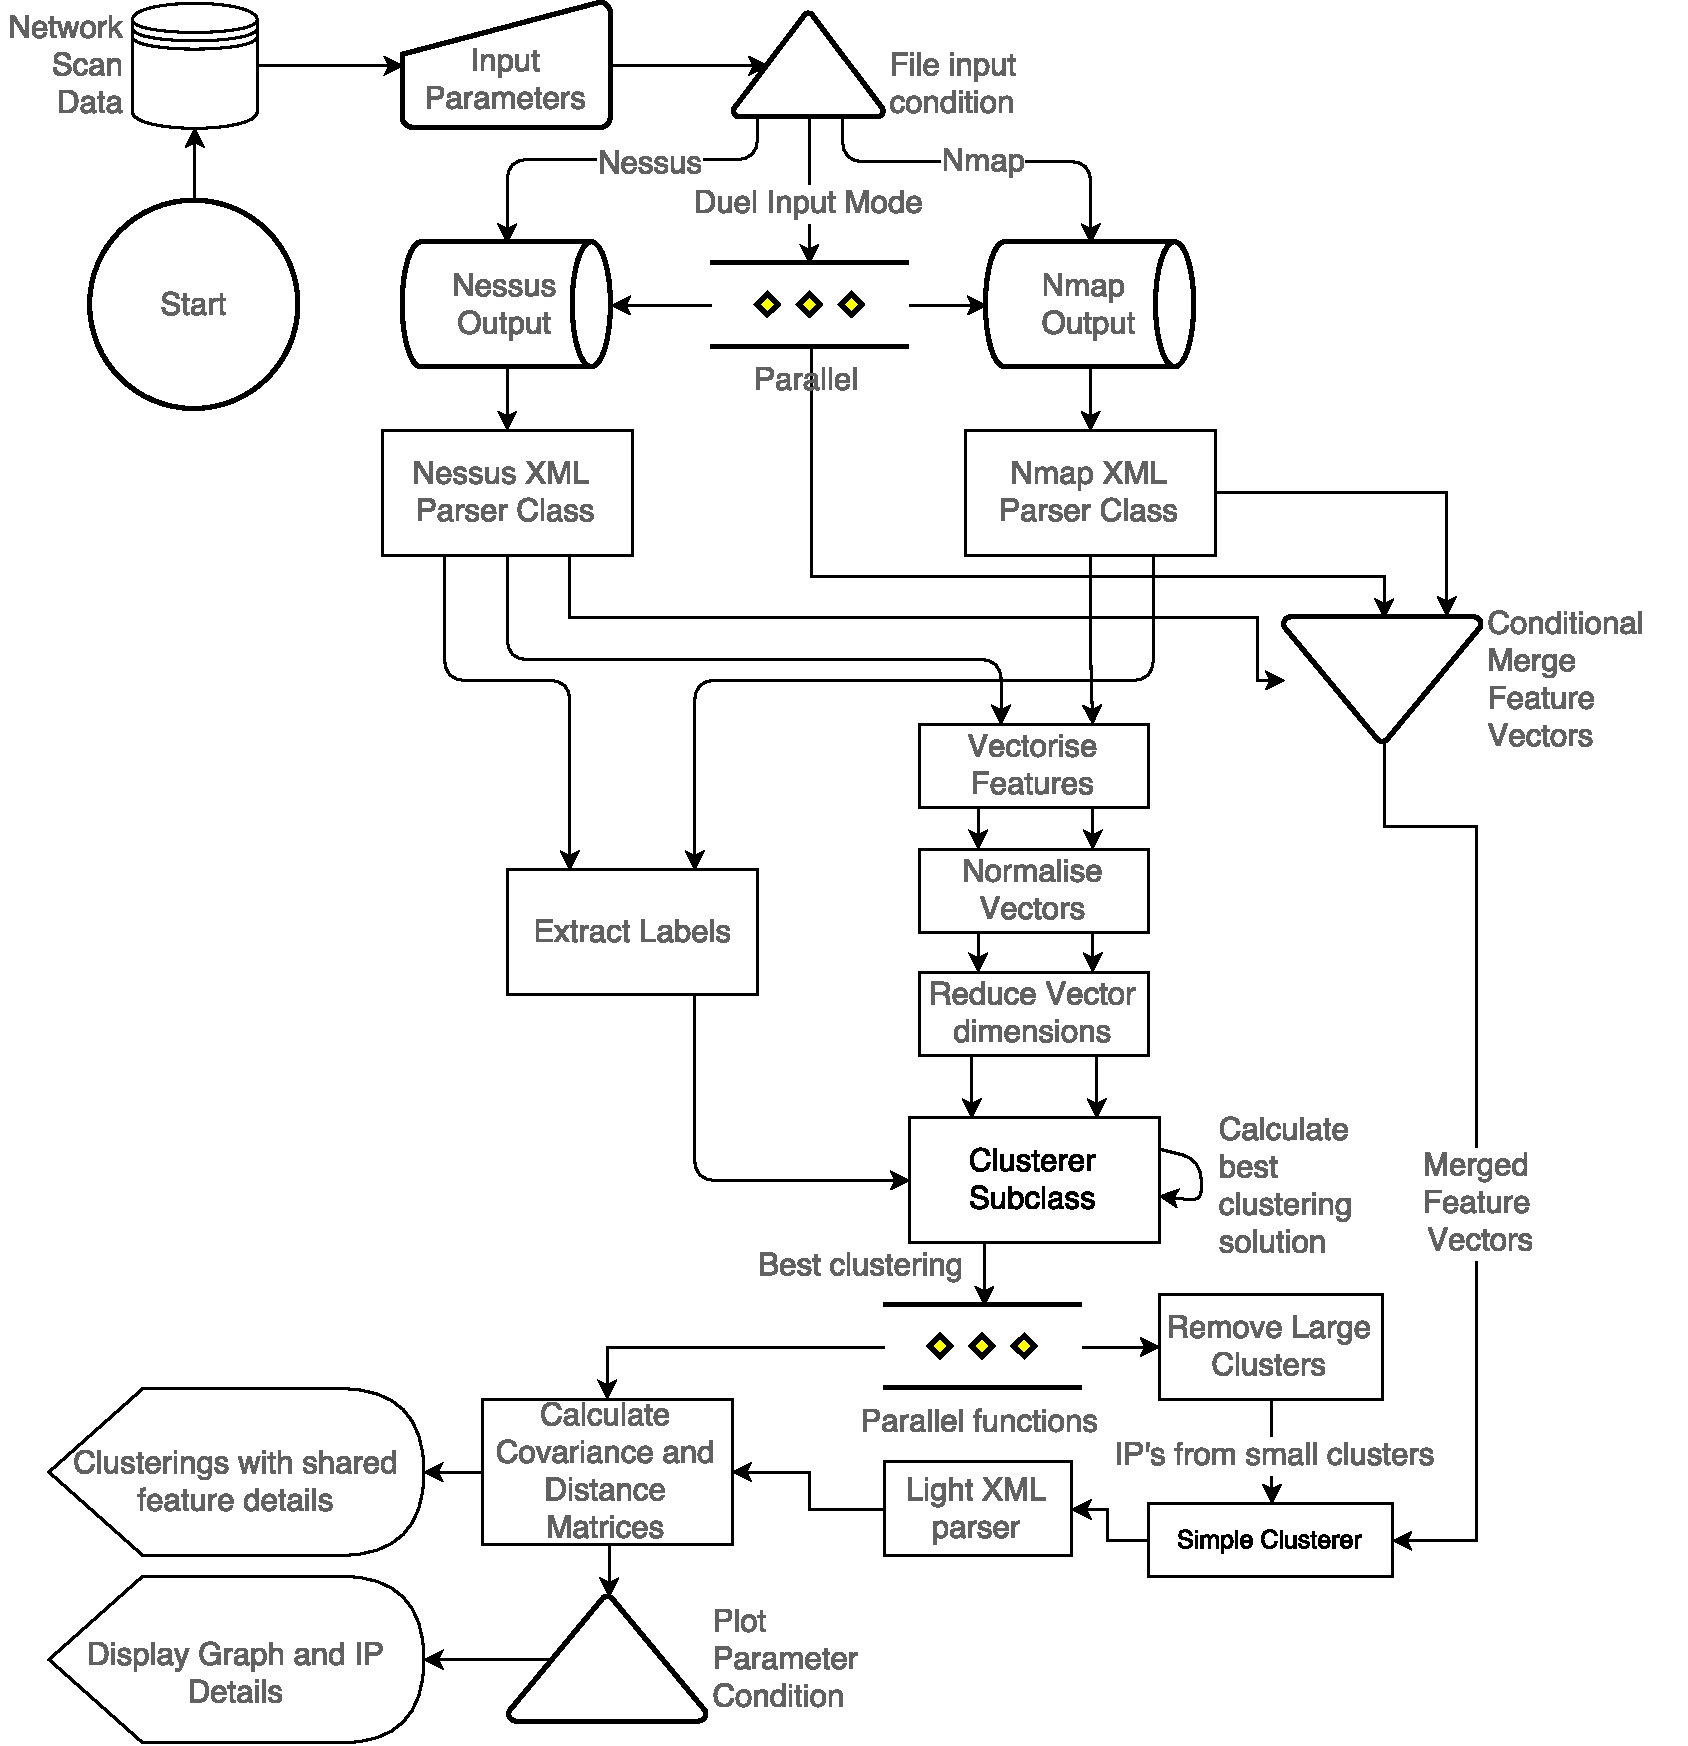
\includegraphics[width=5.5in]{./Figures/flow.pdf}
\caption{Application infrastructure data flow diagram}
\label{flow}
\end{figure}

\paragraph{}Figure \ref{flow} shows the application’s primary class infrastructure when in automatic mode. The infrastructure diagram has been created using standard flow diagram symbols to provide understanding of the process types. The application has been programmed for python version 2.7 interpreters and therefore will not have complete functionality without modification for python 3.0 and above. Due to time constraints placed upon this thesis the library NMAP-Cluster, \cite{blackhatnmap}, was used to conserve time.

\paragraph{}In order to execute this application, it is important to have the correct library dependences. This is done via the python package manager ‘PIP’ and a requirements file, found in Appendix \ref{requirementsfile}, by executing the command:
\lstset{language=Python}
\begin{lstlisting}
Pip install -r requirements.txt
\end{lstlisting}

\paragraph{}The following sections include detailed descriptions of the processes symbolised within the infrastructure Figure \ref{flow}.  Beginning from the start circle and ending at the display modules.\linebreak

\subsection{Usage and Parameters}
\label{infra1}

\begin{figure}[!h]
\centering
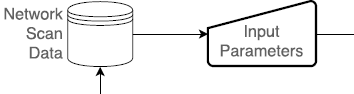
\includegraphics{./Figures/infra1.png}
\caption{Network scan data and input parameter modules from infrastructure diagram at Figure \ref{flow}}
\label{infra1}
\end{figure}

The modules shown in Figure \ref{infra1} are those used to store the network scan data and process the applications input parameters. The Network Scan Data module refers to the XML output of an Nmap scan, Nessus proprietary export file or both. These must be in their respectable formats in order for the parser to recognise them. The files must also be referenced in their correct positional arguments when executing the application such as mentioned in the application usage in Appendix \ref{usage}.

\paragraph{}The Parameters manual input module on Figure \ref{infra1} refers to the parameters that the application requires to select the correct run configuration. This is required because the application has no execution graphical user interface (GUI), the lack of which was decided for several reasons. Such as allowing for scripting, verbose output and terminal pipe operation commands. This type of interface is generally preferred by professionals due to the speed and reliability it provides over a standard GUI. The graphing stage of the application does however, provide a GUI to allow for manipulation of the graphs in multiple ways. The application usage found in Appendix \ref{usage} includes a full description of the possible parameters. The parameters are passed into the data processing section of the application explained in the next session. The three possible run modes are explained in a later section \ref{clustersub}.

\subsection{Data Processing}
\label{infra2}

\begin{figure}[!h]
\centering
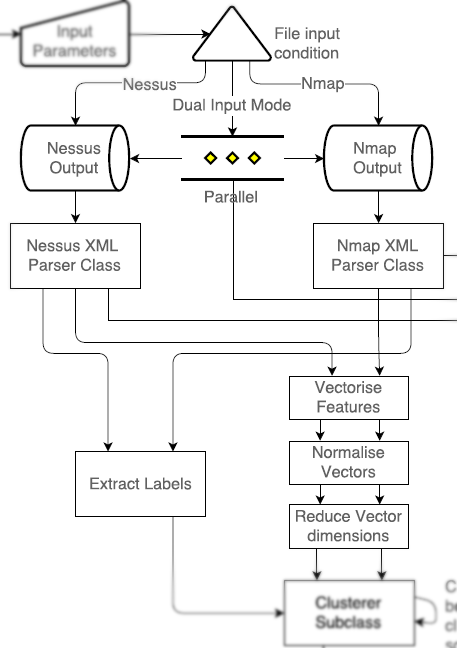
\includegraphics[width=3.5in]{./Figures/infra2.png}
\caption{The data processing section from the infrastructure diagram at Figure \ref{flow} with the irrelevant modules blurred out}
\label{infra2}
\end{figure}
The data processing modules from the infrastructure diagram have been highlighted in Figure \ref{infra2} and will be described in the following paragraphs. \paragraph{}Depending on the files specified within  the input parameters, the application will either feed the Nessus, Nmap or both XML files into the parser classes. These parser classes will take the data from each file and transform it into IP addresses and features which are then passed individually into vectorizers. Vectorization is required for the features to be understood by the clustering algorithm. Vectorization refers to the general process of turning a collection of text (in this case machine attributes) into numerical feature vectors as float values. It is important to note that data from each scanner file is kept separate until the final process. The vectorization class is short and concise due to it having only two purposes, to call the parsers and vectorise the returned results. More information on the vectorization of each file as well as the raw python class code can be found in Appendix \ref{vectorize.py}.

\paragraph{}Once the data has been vectorised it must be normalised in order to avoid large value bias when using dimensionality reduction algorithms such as PCA. Data normalization scales the values to within the same range whilst keeping the data variance and eliminating the bias problem. This is programmed immediately after vectorisation in the applications initialisation class found in its raw code form at Appendix \ref{cluster.py}.

\paragraph{}The major difference between each scanner used is that the Nessus output values include vulnerabilities over Nmap which has superior information on the services and ports of the machine. By using both, the optimal range of information can be achieved, however, this introduces the problem of overfitting which PCA has countered. For more information on PCA refer to dimensionality reduction section \ref{pca} in the introduction. It is possible to greatly modify the output of the two scanners by either using scripts with Nmap or custom plugins for Nessus. Due to the modularity of the application, these modifications to the scanners will not affect the parsers and therefore can be used safely. PCA is also implemented within the initialisation class which can be found in Appendix \ref{cluster.py}. Once PCA is complete, the still separated feature vectors are sent to the clusterer subclass and possibly the conditional merger. The following section will explain the conditional merger of which is represented by symbol in Figure \ref{CMFV}.

\subsection{Small Combined Cluster}
\label{infra3}

\begin{figure}[!h]
\centering
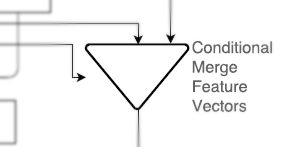
\includegraphics{./Figures/CMFV.png}
\caption{Conditional merge vectors process module from the infrastructure diagram at Figure \ref{flow}}
\label{CMFV}
\end{figure}

\paragraph{}The conditional process of merging the feature vectors, referred to by the symbol in Figure \ref{CMFV}, is executed at this stage, condition dependant on whether dual input mode has been selected when initialising the applications parameters. However, this path must then pause until the main cluster subclass (as represented by the symbol in Figure \ref{clustersub}.) has completed in order to use its clustering outputs. Once this has occurred, each clustering will be duplicated and the large clusters with greater than three IP addresses will be removed from the clustering. This value can be changed based on the network size however the value of three was found to be optimal for networks of size 10 to 1000 from the algorithm tuning stage (this number can be configured for the user’s needs by modifying a single variable ‘maxaddresses’ within the display class highlighted in Figure \ref{ipno} below). The result of each is combined then re-clustered and the remaining IP’s passed through a simpler file parser (compared to that of the ones previously used) to retrieve the information in an un-vectorised text format. This is done to display individual machine information for the end user within the graphing interface. The clustering of these small cluster IP addresses uses the gap statistic (or Elbow method if preferred by user) algorithm to define the numbers of clustered required as appose to user input as these IP’s depend on the cluster subclass’ algorithm calculated clustering. The main cluster subclass mentioned is explained in the following section \ref{infra4}. Gap statistic and Elbow method formulas can be found in the mathematical model at section \ref{models}.

\begin{figure}[!h]
\centering
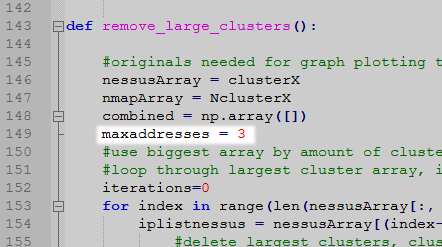
\includegraphics{./Figures/ipno.png}
\caption{Location of the variable which defines the number of maximum IP addresses a cluster is allowed to have for the vulnerability analysis process. The variable is defined within the display.py class’s remove large clusters function on line 149}
\label{ipno}
\end{figure}


\subsection{Clustering Algorithm}
\label{infra4}

\begin{figure}[!h]
\centering
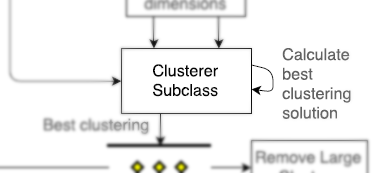
\includegraphics{./Figures/clustersubclass.png}
\caption{Representation of clusterer subclass from infrastructure diagram Figure \ref{flow} spotlighted}
\label{clustersub}
\end{figure}

\paragraph{}The Clusterer subclass represented in the infrastructure diagram by the module in Figure \ref{clustersub}, is where the majority of the calculations are done within the application. This includes the three different modes; manual, assisted and automatic. The raw python code for this module can be found in Appendix \ref{cluster_subclass}. Each mode can be used with a variety of clustering algorithms such as K-means, DBscan and agglomerative clustering. When using dual input mode these functions will execute twice Nessus starting first. A brief summary of each mode is given in the following paragraphs whilst an in-depth algorithm review can be found in section \ref{models}:

    \textbf{Manual:}
     The user supplies all required information to do the clustering. This includes the clustering algorithm and its hyper parameters. If no cluster count ‘K’ is provided and K-means was selected, the gap statistic method will be used to calculate the optimal cluster count. An implementation of the elbow method is also included in the application and can be used instead if the gap statistic if the user desires.

    \textbf{Assisted:}
     The user assists the algorithm by suggesting that some samples should or should not be clustered together. This is a much slower process than the other modes but provides the user with complete control over the clustering decisions. The user must specify the clustering algorithm to use from the selection mentioned above when using this mode.

    \textbf{Automatic:}
     Multiple clustering strategies and parameters are used in an attempt to get the best clustering. Unfortunately, this function can only use the K-means clustering algorithm whilst running in dual input mode, due to limitations of the ‘sklearn’ library’s centroid functions and the time constraints limiting this development as future work. This function goes through each possible iteration of each clustering algorithm up to a maximum cluster value equalling the number of labels in the given dataset. For e.g. in a dataset with ten IP addresses, the maximum allowed clusters is also then. There are multiple selections the user can decide on in terms of which clustering the application will select. This is calculated via a sorting function in the clustering subclass where the user can select between the average silhouette* value, the minimum silhouette* value, the average distance between IP addresses (Euclidian distance by default), the number of clusters in the clustering or the minimum number of common shared features a cluster has in its clustering. These options can also be joined together to make multiple filters. By default, the application uses both the minimum common features and number of overall clusters as filters allowing it to find the clustering with the least number of clusters requiring at least one shared feature. This option is changed near the end of the cluster subclass, changed by uncommenting one line per filter. Each clustering iteration in this loop will calculate the shared positive, negative features, the individual silhouette values and the mean distance to give an overall/per cluster score. Once the iterations are complete for each clustering algorithm the scores and details are used to select one of the clustering’s based on the filters and then it is displayed. When using dual input mode, the vulnerability detection on the small clusters explained above in section \ref{CMFV} is continued, due to it requiring these clusters as input. An example of the full text output and graphing interface for the application’s automatic mode can be found at Appendix \ref{fictional}.\linebreak
\paragraph{}* The silhouette value is used to validate the consistency of clusters in a clustering by indicating whether there are too many or too few clusters. It provides a value of negative one to positive one indicating how well each IP fits in the cluster.  A high value close to one indicates a good clustering by showing that the IP address is very similar to the other IP addresses in its cluster, whilst being very different to the IP addresses of the neighbouring clusters. Therefore, having a low or negative silhouette value indicates the wrong number of clusters used. The silhouette value has been calculated using the Euclidian distance (described in section \ref{KNN}) within the validation class.
     
\subsection{Covariance and Distance Matrices}
\label{infra5}

\begin{figure}[!h]
\centering
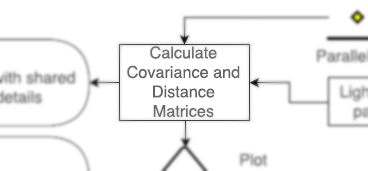
\includegraphics{./Figures/cov.png}
\caption{Representation of covariance and distance matrices function from infrastructure diagram Figure \ref{flow} spotlighted}
\label{cov}
\end{figure}

\paragraph{}Covariance and distance matrices are calculated just before displaying the graphing interface. The function symbol is shown in Figure \ref{cov} above. The output from these functions can be found at the end of the text output, an example is shown in Appendix \ref{exampleoutput}. This is shown for the purpose of giving a technical user greater knowledge of the data-set used which can be interpreted and reported to the client in a security assessment. Specifically, the covariance matrix shows how related the centroids for each clustering are to each other, in other words, their similarity. Covariance will highlight any linear relationships that might be apparent within the dataset with the values ranging from negative one to positive one, high values indicating a positive linear relationship. The Distance matrix shows the literal Euclidian distance between each clustering centroid but by design that also correlates to showing a numericized value defining how different the clusters are from each other. These calculations are done for each clustering result in the current mode (For e.g. three times if using dual mode), however, they are only shown in verbose level one and above modes.

\subsection{Display and Output Modules}
\label{infra6}

\begin{figure}[!h]
\centering
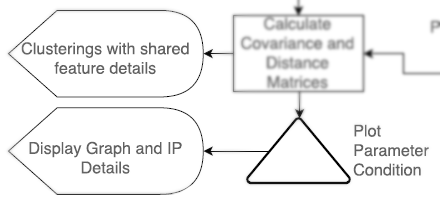
\includegraphics{./Figures/display.png}
\caption{Representation of the display modules from infrastructure diagram Figure \ref{flow} with irrelevant modules blurred out}
\label{display}
\end{figure}

The application will display the main output at the end of its execution as shown in the infrastructure diagram with the symbol from Figure \ref{display}. The application will show a running output as the calculations and cluster iterations are performed, providing that the verbosity level is set to one or higher. The verbosity parameter will only effect the text output and not the graphing interface of the application which will remain identical, an example of full text output using dual mode can be found at \ref{exampleoutput}. Without verbose output selected the text output will only show the cluster details (for both formats if using dual mode). In order for the application to display the graphing interface on clustering class completion the application must be run with the parameter ‘-p’ as mentioned in the usage descriptor found in \ref{usage}. The graphs displayed within the graphing GUI are fully manipulatable with zoom, pan and save as functions, however, the graphing interface will differ depending on which mode the application is using. \linebreak
\paragraph{}\textbf{dual mode} graphing interface will display five graphs and a small text segment underneath the bottom graph. The five segments are arranged in a grid of 4 with a large graph beneath the grid spanning both columns as the 5th. The first row of two graphs displays the Nmap output with the right graph solely displaying the centroids and the left displaying the entire Nmap clustering with IP addresses. The second row displays the Nessus graphs in the same configuration as Nmap above. The 3rd row graph displays the IP addresses from the clusters with less than 3 IP addresses (this value is the default and can be changed by following the instruction described in section \ref{CMFV} and Figure \ref{ipno}). The reason for why this is done has been explained within the application brief at section \ref{brief} and the method used explained within section \ref{CMFV}. The text segment beneath the 3rd row graph displays the detected operating system information and the probability of that detection being true. This is shown for each IP address in the small cluster IP addresses graph just above the text segment. An example of the dual mode graphing interface can be found in Figure \ref{example_dual} and Figure \ref{dual}.\linebreak
\paragraph{}\textbf{Standard mode} graphing interfaces are similar to each other as they contain the same two graph split with just different information. The graphs are similar to that of dual mode without the small combined cluster graph of which the left graph includes the full clustering with IP addresses and the right graph solely contains the centroids of those clusters. Two examples of this mode can be found in the Appendix as Figure \ref{split_nessus} for Nessus clustering and Figure \ref{split_nmap} for Nmap clustering, along with the commands used to achieve them. 



\section{Mathematical Model and Algorithms}
\label{models}

\paragraph{}The following information consists of mathematical representations for the modules in the applications primary class architecture, as shown in figure \ref{flow}.
Parse XML files into matrices V for each input file, consisting of two dimensions’ \textit{m} and \textit{n} respectively. The matrices are then vectorised from JSON strings outputted from the parser classes into numerical float representations.
These matrices' data is then normalized using the following formula denoted in the journal of Normalization: A Preprocessing Stage, \cite{normalization}.:
Where Vn is the nth¬ dimension of matrix V and contains the features for each label Vm.

${V_n} = \frac{{({V_n} - \;\min \left\{ {{V_n}} \right\})}}{{\left( {\max \left\{ {{V_n}} \right\} - \min \left\{ {{V_n}} \right\}} \right)}}\left( {ne{w_{\max \left\{ {{{\rm{V}}_{\rm{n}}}} \right\}}} - ne{w_{{\rm{min}}\left\{ {{V_n}} \right\}}}} \right) + new\_{\rm{min}}\left\{ {{V_n}} \right\}$% MathType!End!2!1!

This application will normalise the data to the range of 0 to 1 in which the formula is adjusted to the following:

${V_n} = \frac{{({V_n} - \;\min \left\{ {{V_n}} \right\})}}{{\left( {\max \left\{ {{V_n}} \right\} - \min \left\{ {{V_n}} \right\}} \right)}}$% MathType!End!2!1!


\paragraph{}The Vn dimension of matrix V of each input file is then passed through a principle component analysis formula for dimensionality reduction to two dimensions. This is due to the current number of dimension layers directly correlating to a feature of which there is an average of three hundred per IP address (or \textit{Vm}). This is calculated by using the SKlearn PCA decomposition library which uses the probabilistic model of PCA defined in the journal of Probabilistic Principle Component Analysis, \cite{probabilityPCA}. This algorithm is too complex to be included within the scope of this thesis and therefore is not described here. The result of this PCA algorithm returns a new matrix with two dimensions, which is then used in the K-means clustering algorithm as input with the IP address labels (or \textit{Vm}).

\paragraph{}The standard Lloyd’s algorithm for K-means clustering was then used against the PCA output vectors which can be described as the following five stages. This is carried out for each clustering iteration in the cluster class depending on its current mode.

\begin{enumerate}
\item Clusters the Vectors inputs into K number of clusters where K is either assigned manually, iteratively or calculated using the Gap statistic and Elbow values explained below. This depends on the current application mode and user parameters at run time.
\item  Select K number of points at random locations to act as cluster centroids.
\item  Assign objects to their closest plotted centroid per the selected distance function (Euclidian as default).
\item Calculate the new centroid for each cluster in this new clustering.
\item Repeat steps 2, 3 and 4 until the same points are assigned to each cluster in consecutive rounds and no changes are present in the clustering. In the case of automatic mode, the K value will increment up to a maximum equalling the number of IP addresses or labels in Vm.
\end{enumerate}

\paragraph{}However, the user can also select the use of DBscan or Agglomerative clustering algorithms instead of K-means for any mode apart from dual input. However, due to the limited usage they provide for the applications design goals, will not be described in this thesis. 

\paragraph{}Each clustering result of this algorithm has several calculations carried out upon it in order to validate and provide scores to the clustering. These calculations are denoted in section \ref{clustersub}. The primary function used to score these clustering’s is a silhouette value which has been defined in the journal, Silhouettes: A graphical aid to the interpretation and validation of cluster analysis, \cite{silhouette}. A full description of what this value provides for the user is included at the end of section \ref{clustersub}. The formulas used to calculate the silhouette value are taken from the previously mentioned journal and are described below.

\paragraph{}For each vector \textit{i}, \textit{a(i)} would be the average dissimilarity of vector \textit{i} with all other vectors within the same cluster. \textit{b(i)} is the lowest average dissimilarity of vector \textit{i} to any other cluster of which vector \textit{i} is not a member of. The cluster with the lowest value for \textit{b(i)} is the closest neighbouring cluster and therefore the most similar. This defines the following formula for silhouette value \textit{s(i)}.\linebreak
$s\left( i \right) = \frac{{b\left( i \right) - a\left( i \right)}}{{\max \left\{ {a\left( i \right),b\left( i \right)} \right\}}}$


\paragraph{}The resulting clustering’s are sorted based on the filters mentioned in \ref{clustersub} and the best clustering is chosen. This best clustering is passed through into the small combined cluster algorithm described in section \ref{CMFV} as well as the display class in \ref{display}.

\paragraph{}When the application uses the K-means clustering algorithm and a value for K is not defined, the application will attempt to calculate the optimal value for K via either the Gap Statistic or Elbow value methods depending on the user’s preferences. This is changed within the optimal k means class with the default value being the Gap Statistic method. The python implementation of the Gap Statistic method can be found in the Appendix \ref{gapstatistic} with the formulas used were originally developed by Stanford researchers from the journal, Estimating the number of clusters in a data set via the gap statistic, \cite{gapref}. The implementation of the researchers’ algorithm within this application can be described by the following points.

\begin{enumerate}

\item Cluster the data via K-means from the range of k=1 to k=max and calculate the variance quantity variable \textit{Wk} (primarily used for elbow method).
\item Generate the reference data sets \textit{B} and cluster them with the same k values as previous step. 
\item Calculate the gap statistic value with the following formula: \linebreak
$Gap\left( k \right) = \left( {\frac{1}{B}} \right)\mathop \sum \limits_{b = 1}^B logW_{kb}^* - log{W_k}.$
\item Calculate the standard deviation using: \linebreak
$sd\left( k \right) = {\left[ {\left( {\frac{1}{B}} \right)\mathop \sum \limits_b (logW_{kb}^* - {{(\left( {\frac{1}{B}} \right)\mathop \sum \limits_b logW_{kb}^*)}^2}} \right]^{1/2}}$
\item Then define ${s_k} = \;\sqrt {1 + \frac{1}{B}} sd\left( k \right)$ which allows the optimal number of K to be the smallest k such that $Gap\left( k \right) \ge Gap\left( {k + 1} \right) - {s_{k + 1}}$. 

\end{enumerate}

The Covariance and distance matrices displayed prior to graphing output are calculated using the following methods. More information on these values can be found in \ref{infra5}.
Covariance for a given centroid vector dimensions \textit{x} and \textit{y} is calculated using the formula: $cov\left( {x,y} \right) = \frac{{(\mathop \sum \nolimits_{i = 1}^n \left( {{x_i} - \bar x} \right)\left( {{y_i} - \bar y} \right))\;}}{{n - 1}}$ . This is calculated for each centroid in the chosen clustering and displayed in a matrix.
The distance matrix displays the Euclidian distance between the x and y values for each centroid in the clustering.

\section{Application Testing}
\label{testing}
\paragraph{}Unfortunately due to the sensitive nature of the data required by the application, there are no datasets to be found publicly available online. Therefore, in order to design a proof of concept test procedure a dataset must be created using a significant network size to simulate the proportions of a real organizational network. The size requirements of this dataset limit the use of virtualized machine networks due the raw processing power required for a network of that size, hence, the permission was granted to allow for the scanning of a private network laboratory in the University of Abertay. The laboratory consisted of approximately 50 online devices at the time of scanning. The raw scan output files for Nmap and Nessus can be found within the thesis’ artefacts, hacklab analysis folder with the file names hacklab\_new.xml and hacklab\_new.nessus respectfully.

\paragraph{}The creation of this dataset required installing the Nmap and Nessus scanner tools on a separate device plugged into the network for this sole purpose. The device used to enter the network and execute the scans was a Dell latitude E6410 laptop running the latest rolling release kernel of Arch Linux. This setup was used specifically to replicate a similar scenario to that of what an industry professional might encounter. The latest stable releases of the required software were used. At the time of writing this thesis (April 2017) those reference numbers were as follows: 
\begin{itemize}
\item Nmap 7.40
\item Nessus 6.10.5 
\item Python 2.7.13
\item Python Libraries
\begin{itemize}
\item backports-abc==0.4
\item bokeh==0.12.1
\item certifi==2016.8.8
\item cycler==0.10.0
\item futures==3.0.5
\item Jinja2==2.8
\item MarkupSafe==0.23
\item matplotlib==1.5.1
\item numpy==1.11.1
\item pyparsing==2.1.8
\item python-dateutil==2.5.3
\item pytz==2016.6.1
\item PyYAML==3.11
\item requests==2.11.0
\item scikit-learn==0.17.1
\item scipy==0.18.0
\item singledispatch==3.4.0.3
\item six==1.10.0
\item tornado==4.4.1
\item tabulate==0.7.7
\end{itemize}
\end{itemize}

The Nmap scan was created using the following command: 
\begin{lstlisting}[language=python]
nmap -A -O -oX hacklab.xml 10.0.0.0/24
\end{lstlisting}
The -Ox flag in this command exports the scan as an XML which is the only export format the clustering application currently supports.\linebreak
The Nessus scan was created by using the default scan policy in the advanced scan mode with the same scope as nmap, 10.0.0.0/24. This was then exported as the latest version of the proprietary Nessus XML format from the scan overview page.

\paragraph{}Once both scans have completed the next step is to remove the testing device used from the XML files manually due to each scanner retrieving greatly differing results from the testing machine compared to other machines on the network. This step is crucial and ignoring it will manipulate the final result of the clustering algorithm rendering it inaccurate. The artefact files have had this step done prior to submission.

The scan files have then been passed through the clustering application using the following commands for each input type in automatic mode:\linebreak

\textbf{Nmap}
\begin{lstlisting}[language=bash]
cluster.py -s automatic -vv -p "../hacklab analyses/hacklab_new.xml"
\end{lstlisting}

\textbf{Nessus}
\begin{lstlisting}[language=bash]
cluster.py -s automatic -vv -p -N "../hacklab analyses/hacklab_new.nessus"
\end{lstlisting}


\textbf{Dual Input}
\begin{lstlisting}[language=bash]
cluster.py -s automatic -vv -p -t -N -tp "../hacklab analyses/hacklab_new.xml" "../hacklab analyses/hacklab_new.nessus"
\end{lstlisting}

\paragraph{}More information and the results for this proof of concept test can be found in Appendix section \ref{hacklab}. These results will be validated within the thesis conclusions.


